%%%%%%%%%%%%%%%%%%%%%%%%%%%%%%%%%%%%%%%%%%%%%%%%%%%%%%%%%%
% Ping GCM
%%%%%%%%%%%%%%%%%%%%%%%%%%%%%%%%%%%%%%%%%%%%%%%%%%%%%%%%%%
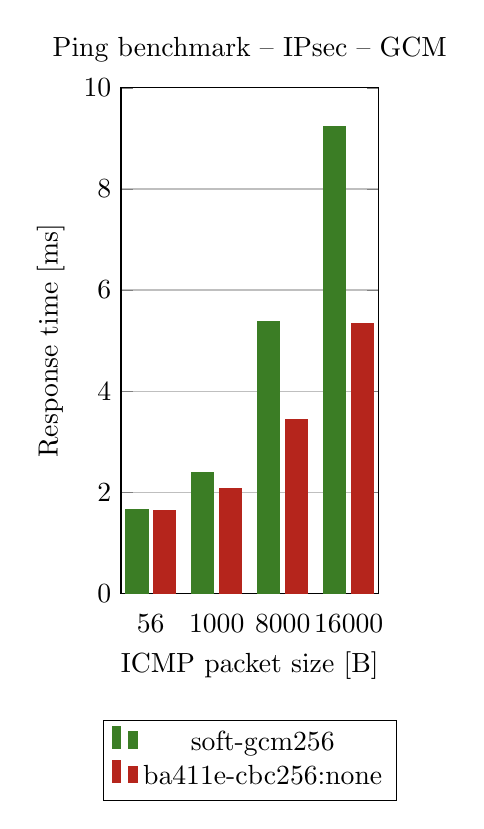
\begin{tikzpicture}
\begin{axis}[
        title = {Ping benchmark -- IPsec -- GCM},
        width  = 0.4\textwidth,
        height = 8cm,
        major x tick style = transparent,
        ybar,
        bar width=8pt,
        ymajorgrids = true,
        ylabel = {Response time [ms]},
        xlabel = {ICMP packet size [B]},
        ymin=0, ymax=10,
        symbolic x coords={56, 1000, 8000, 16000},
        xtick = data,
        scaled y ticks = false,%Disable the *10^4 exponent applied to all y axis markings.
        legend style={at={(0.5,-0.25)}, anchor=north,legend columns=1},
        enlarge x limits=0.15,
    ]
% I would have prefered to have "\addplot[marks only]", but they overlap if they have the same x coordinate,
% not like bars that automatically shift.
\addplot[style={OliveGreen, fill=OliveGreen}]
    coordinates {
        (56, 1.651)
        (1000, 2.388)
        (8000, 5.383)
        (16000, 9.241)
    };
    \label{soft-gcm256}

\addplot[style={BrickRed, fill=BrickRed}]
    coordinates {
        (56, 1.639)
        (1000, 2.080)
        (8000, 3.445)
        (16000, 5.345)
    };
    \label{ba411e-cbc256:none}

\legend{soft-gcm256, ba411e-cbc256:none}
\end{axis}
\end{tikzpicture}
% Here, I could show the gcm256, which show better performances with the BA411e, but I would be weird to compare it with aes256cbc.
% I need another graph with a CPu usage comparison to show that even if the perf are the same for soft/hard with aes256gcm, the hard loads less the CPU (I hope so, at least).